\section{Résultats de l'expérimentation}

La dernière étape de ce projet consistait à réaliser des acquisitions à l'aide de la solution développée en partie \ref{sub:ihm}, en suivant les différents cas de tests détaillés en \ref{subsub:test}.

Une routine Python a été conçue pour récupérer les données radar brutes ainsi que le vecteur de position, tout en adaptant le format des données aux exigences de la chaîne de traitement.

La figure \ref{fig:res} présente les données obtenues lors d'une acquisition monocible après l'opération de compression en distance (détaillée en \ref{subsubsec:compression_dist}). Cette matrice est représentée en deux dimensions ainsi que selon un plan de coupe en portée. On y observe une forte concentration d'énergie dans les premiers mètres, phénomène dû au self-mixing. La vue en coupe met clairement en évidence l'absence de focalisation de la cible : lors de la Backprojection, l'intégralité de l'énergie reste concentrée sur les courtes distances.

En l'état, ces expérimentations ne nous permettent pas de former une image, ni de valider notre chaîne de traitement sur des données réelles (qu'il s'agisse de la Backprojection, de la détection ou de l'autofocus). 
\begin{figure}[htbp]
    \centering
    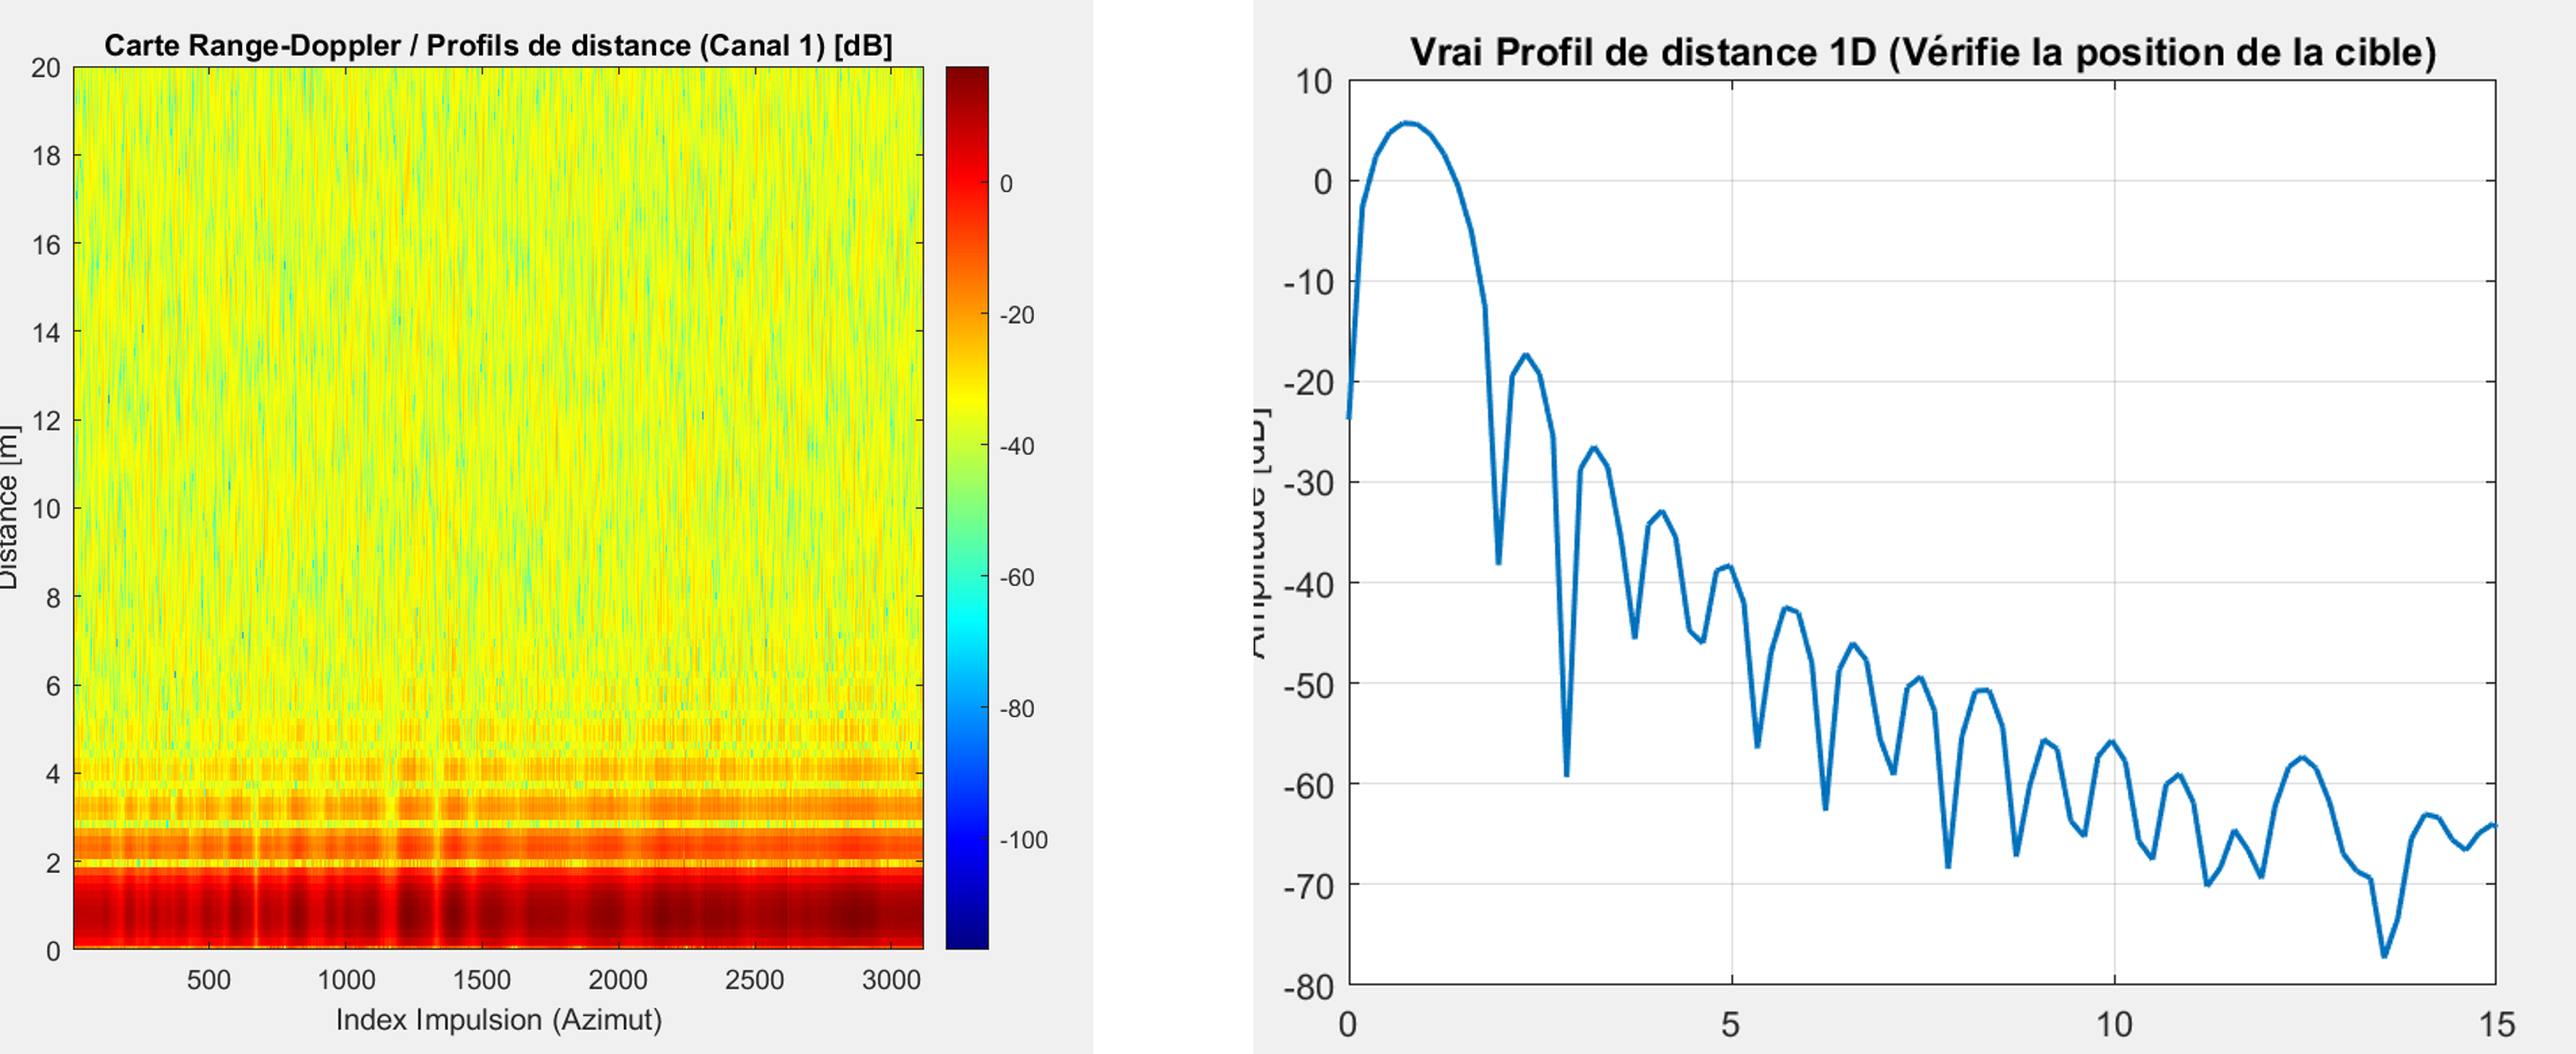
\includegraphics[width=0.9\linewidth]{src/rapport_complet/img/self.png}
    \caption{Visualisation des données après compression en distance (en 2D et vue de coupe en portée)}
    \label{fig:res}
\end{figure}